\documentclass[a4paper,UKenglish,cleveref, autoref, thm-restate]{lipics-v2021}

\hideLIPIcs

\usepackage{amsmath}
\usepackage{numprint}
\npdecimalsign{.} % we want . not , in numbers

\usepackage{xspace}

\newcommand{\codestyling}[1]{\texttt{#1}}
\newcommand{\ie}{i.e.,\xspace~}
\newcommand{\Ie}{I.e.,\xspace~}
\newcommand{\eg}{e.g.,\xspace~}
\newcommand{\Eg}{E.g.,\xspace~}
\newcommand{\etal}{et~al.}

\setlength\parfillskip{0pt plus .4\textwidth}
\setlength\emergencystretch{.1\textwidth}
\clubpenalty10000
\widowpenalty10000
\displaywidowpenalty=10000

\bibliographystyle{plainurl}

\title{Advanced Data Structures: Final Report}
\titlerunning{Final Report}

\author{Steil, Patrick}{2513240}{patrick.steil@student.kit.edu}{}{}
\authorrunning{Steil, Patrick}

\Copyright{P. Steil}

\keywords{Predecessor, Range Minimum Queries} %TODO mandatory; please add comma-separated list of keywords
\category{}
\relatedversion{}

\begin{CCSXML}
<ccs2012>
   <concept>
       <concept_id>10003752.10003809.10010031</concept_id>
       <concept_desc>Theory of computation~Data structures design and analysis</concept_desc>
       <concept_significance>100</concept_significance>
       </concept>
 </ccs2012>
\end{CCSXML}

\ccsdesc[100]{Theory of computation~Data structures design and analysis}

\supplementdetails[subcategory={Code}]{Software}{https://github.com/PatrickSteil/BitDatastructures}

%\nolinenumbers %uncomment to disable line numbering

%Editor-only macros:: begin (do not touch as author)%%%%%%%%%%%%%%%%%%%%%%%%%%%%%%%%%%
\EventEditors{}
\EventNoEds{0}
\EventLongTitle{}
\EventShortTitle{}
\EventAcronym{}
\EventYear{0}
\EventDate{0}
\EventLocation{}
\EventLogo{}
\SeriesVolume{0}
\ArticleNo{0}
%%%%%%%%%%%%%%%%%%%%%%%%%%%%%%%%%%%%%%%%%%%%%%%%%%%%%%

\begin{document}
	
	\maketitle
	
	%\section{Introduction}
	%\label{sec:introduction}
	\begin{abstract}
	In this work, different data structures are implemented that can efficiently answer two types of queries: predecessor and range-minimum queries. For this purpose, the Elias-Fano coding and several “Block-Lookup” data structures are implemented and tested. The project is part of the “Advanced Data Structures” lecture at KIT in the summer semester 2023 with Dr.~Florian Kurpicz.
	\end{abstract}
	\section{Algorithms and Data Structures (DS)}
	\label{sec:algorithms}
	\paragraph*{Predecessor Data Structures}
	Predecessor data structures are unique data structures developed to efficiently solve the problem of predecessor access. The predecessor access problem is to find the predecessor (the element with the highest value that is less than a given element) in a set of elements.
	Without additional memory consumption, elements can be stored sorted or in a binary search tree, whereby a predecessor query can subsequently be answered with a runtime of~$\mathcal{O}\left(\log(n)\right)$. However, this is too slow in practice, which is why techniques such as \textit{x/y-fast-tries}~\cite{WILLARD198381} or \textit{Elias-Fano encoding}~\cite{10.1145/321812.321820} have been developed. The idea of the last technique is to divide the representation of numbers into two parts, on the one hand, the \textit{most significant} bits with a length of~$\left\lceil\log\left(n\right)\right\rceil$ and on the other hand the remaining bits. This way, all numbers with the same \textit{most significant} bits are ``grouped'' during a query, meaning a query only has to look at one ``group'' of numbers. However, this may result in all numbers being scanned if the numbers are not favourable.	
	\paragraph*{Range-Minimum Queries}
	Range minimum queries (RMQ) refer to a particular type of search operation in data structures where the minimum value within a given interval (range) of elements in a set is to be found. The goal is to efficiently find the biggest value smaller than a given element among a subset of elements. Analogous to the predecessor data structures, trade-offs exist between additional memory and runtime (the different pre-computation times can be neglected for static data). To answer RMQ quickly, one can use~$\Theta\left(n^2\right)$ additional memory to calculate all possible queries in advance and thus obtain a constant query time (only a memory access). One can now only precompute queries of specific ranges to reduce the impractical quadratic memory. If the size of this range is cleverly chosen, one obtains constant query time and down to only linear additional memory.
	
	\section{Implementation}
	
	\paragraph*{Elias-Fano}
	For an efficient Elias-Fano implementation, one needs a bit-vector data structure that can efficiently answer \textsc{select} query. The current Elias-Fano data structure consists of two bit vectors: \textit{upperBits} and \textit{lowerBits}. The former encodes in~$2n+1$ bits the \textit{most significant bits} (MSB) of the numbers, and in \textit{lowerBits}, the remaining bits (LSB) of the numbers are stored straightforwardly. Please see Appendix~\ref{app:sec::ef} on the ``minor'' Elias-Fano Problem, which I mentioned in person. Otherwise, my implementation of \textsc{predecessor} is based on the description of~\cite{pibiri2020succinct}. To identify the predecessor of the number~$x$, I use \textsc{select} queries to find the ``leftmost'' and ``rightmost'' index of numbers for which the MSB is equal to the MSB of~$x$. Subsequently, scanning this range to find the predecessor is straightforward.

	\paragraph*{Range-Mimimum Queries}
	For the range-minimum queries, I implemented all 3 data structures, \ie the one with~$\mathcal{O}\left(n^2\right)$, ~$\mathcal{O}\left(n \log\left(n\right)\right)$ and the one with~$\mathcal{O}\left(n\right)$ additional memory. I have not implemented the latter data structure precisely as in the lecture; namely, I have not implemented the \textit{Cartesian Trees}. Instead, I have split the query into three parts. I check which parts of the given range are ``covered'' by blocks and then scan the initial and final part (from the left index to the first ``completely covered'' block and analogously from the last covered block to the end) and the covered blocks. The initial and final check is usually done with Cartesian trees; I have implemented a linear search over the part of the array. Note that this approach is very cache-efficient and for small enough ranges faster than using Cartesian trees.
	
	\section{Experiments}
	%\subsection{Hardware \& Code}
	The programming language used was \codestyling{C++}, and the compiler was \codestyling{G++} with optimisations enabled. All experiments were conducted on a ThinkCentre running Ubuntu 22.10 with an \codestyling{Intel(R) Core(TM) i5-8500T CPU} @ 2\,.10GHz processor.
	\paragraph*{Elias-Fano}
	The performance (based on the provided benchmarks) of the Elias-Fano encoding can be seen in Figure~\ref{fig:ef}. It can be noticed that both the memory consumption and the query depend on the distribution of the numbers. In the first file, \numprint{1000000} numbers are present in the \textit{total} range of~$\left[0, 2^{64}\right)$, \ie scattered throughout the universe. On the other hand, in the file \textit{File 2}, only ``small'' numbers are present, \ie very one-sidedly distributed in the universe. If one would not resize the universe to the maximum number occuring in the given set, basically all MSB are 0 for all numbers, resulting in no speedup compared to linear search.
	\begin{figure}[htbp]
		\begin{center}
			\resizebox{.9\linewidth}{!}{
				% GNUPLOT: LaTeX picture with Postscript
\begingroup
  \makeatletter
  \providecommand\color[2][]{%
    \GenericError{(gnuplot) \space\space\space\@spaces}{%
      Package color not loaded in conjunction with
      terminal option `colourtext'%
    }{See the gnuplot documentation for explanation.%
    }{Either use 'blacktext' in gnuplot or load the package
      color.sty in LaTeX.}%
    \renewcommand\color[2][]{}%
  }%
  \providecommand\includegraphics[2][]{%
    \GenericError{(gnuplot) \space\space\space\@spaces}{%
      Package graphicx or graphics not loaded%
    }{See the gnuplot documentation for explanation.%
    }{The gnuplot epslatex terminal needs graphicx.sty or graphics.sty.}%
    \renewcommand\includegraphics[2][]{}%
  }%
  \providecommand\rotatebox[2]{#2}%
  \@ifundefined{ifGPcolor}{%
    \newif\ifGPcolor
    \GPcolorfalse
  }{}%
  \@ifundefined{ifGPblacktext}{%
    \newif\ifGPblacktext
    \GPblacktexttrue
  }{}%
  % define a \g@addto@macro without @ in the name:
  \let\gplgaddtomacro\g@addto@macro
  % define empty templates for all commands taking text:
  \gdef\gplbacktext{}%
  \gdef\gplfronttext{}%
  \makeatother
  \ifGPblacktext
    % no textcolor at all
    \def\colorrgb#1{}%
    \def\colorgray#1{}%
  \else
    % gray or color?
    \ifGPcolor
      \def\colorrgb#1{\color[rgb]{#1}}%
      \def\colorgray#1{\color[gray]{#1}}%
      \expandafter\def\csname LTw\endcsname{\color{white}}%
      \expandafter\def\csname LTb\endcsname{\color{black}}%
      \expandafter\def\csname LTa\endcsname{\color{black}}%
      \expandafter\def\csname LT0\endcsname{\color[rgb]{1,0,0}}%
      \expandafter\def\csname LT1\endcsname{\color[rgb]{0,1,0}}%
      \expandafter\def\csname LT2\endcsname{\color[rgb]{0,0,1}}%
      \expandafter\def\csname LT3\endcsname{\color[rgb]{1,0,1}}%
      \expandafter\def\csname LT4\endcsname{\color[rgb]{0,1,1}}%
      \expandafter\def\csname LT5\endcsname{\color[rgb]{1,1,0}}%
      \expandafter\def\csname LT6\endcsname{\color[rgb]{0,0,0}}%
      \expandafter\def\csname LT7\endcsname{\color[rgb]{1,0.3,0}}%
      \expandafter\def\csname LT8\endcsname{\color[rgb]{0.5,0.5,0.5}}%
    \else
      % gray
      \def\colorrgb#1{\color{black}}%
      \def\colorgray#1{\color[gray]{#1}}%
      \expandafter\def\csname LTw\endcsname{\color{white}}%
      \expandafter\def\csname LTb\endcsname{\color{black}}%
      \expandafter\def\csname LTa\endcsname{\color{black}}%
      \expandafter\def\csname LT0\endcsname{\color{black}}%
      \expandafter\def\csname LT1\endcsname{\color{black}}%
      \expandafter\def\csname LT2\endcsname{\color{black}}%
      \expandafter\def\csname LT3\endcsname{\color{black}}%
      \expandafter\def\csname LT4\endcsname{\color{black}}%
      \expandafter\def\csname LT5\endcsname{\color{black}}%
      \expandafter\def\csname LT6\endcsname{\color{black}}%
      \expandafter\def\csname LT7\endcsname{\color{black}}%
      \expandafter\def\csname LT8\endcsname{\color{black}}%
    \fi
  \fi
    \setlength{\unitlength}{0.0500bp}%
    \ifx\gptboxheight\undefined%
      \newlength{\gptboxheight}%
      \newlength{\gptboxwidth}%
      \newsavebox{\gptboxtext}%
    \fi%
    \setlength{\fboxrule}{0.5pt}%
    \setlength{\fboxsep}{1pt}%
    \definecolor{tbcol}{rgb}{1,1,1}%
\begin{picture}(7200.00,5040.00)%
    \gplgaddtomacro\gplbacktext{%
      \csname LTb\endcsname%%
      \put(1342,440){\makebox(0,0)[r]{\strut{}$0$}}%
      \put(1342,1003){\makebox(0,0)[r]{\strut{}$5\times10^{8}$}}%
      \put(1342,1565){\makebox(0,0)[r]{\strut{}$1\times10^{9}$}}%
      \put(1342,2128){\makebox(0,0)[r]{\strut{}$1.5\times10^{9}$}}%
      \put(1342,2691){\makebox(0,0)[r]{\strut{}$2\times10^{9}$}}%
      \put(1342,3254){\makebox(0,0)[r]{\strut{}$2.5\times10^{9}$}}%
      \put(1342,3816){\makebox(0,0)[r]{\strut{}$3\times10^{9}$}}%
      \put(1342,4379){\makebox(0,0)[r]{\strut{}$3.5\times10^{9}$}}%
      \put(2553,220){\makebox(0,0){\strut{}ex1.txt}}%
      \put(3633,220){\makebox(0,0){\strut{}ex2.txt}}%
      \put(4712,220){\makebox(0,0){\strut{}ex3.txt}}%
      \put(5923,440){\makebox(0,0)[l]{\strut{}$200$}}%
      \put(5923,1097){\makebox(0,0)[l]{\strut{}$400$}}%
      \put(5923,1753){\makebox(0,0)[l]{\strut{}$600$}}%
      \put(5923,2410){\makebox(0,0)[l]{\strut{}$800$}}%
      \put(5923,3066){\makebox(0,0)[l]{\strut{}$1000$}}%
      \put(5923,3723){\makebox(0,0)[l]{\strut{}$1200$}}%
      \put(5923,4379){\makebox(0,0)[l]{\strut{}$1400$}}%
    }%
    \gplgaddtomacro\gplfronttext{%
      \csname LTb\endcsname%%
      \put(209,2409){\rotatebox{-270}{\makebox(0,0){\strut{}Space [bits]}}}%
      \put(6693,2409){\rotatebox{-270}{\makebox(0,0){\strut{}Time [ms]}}}%
      \csname LTb\endcsname%%
      \put(4804,4206){\makebox(0,0)[r]{\strut{}Space [bits]}}%
      \csname LTb\endcsname%%
      \put(4804,3986){\makebox(0,0)[r]{\strut{}Time [ms]}}%
      \csname LTb\endcsname%%
      \put(3632,4709){\makebox(0,0){\strut{}Space and Time}}%
    }%
    \gplbacktext
    \put(0,0){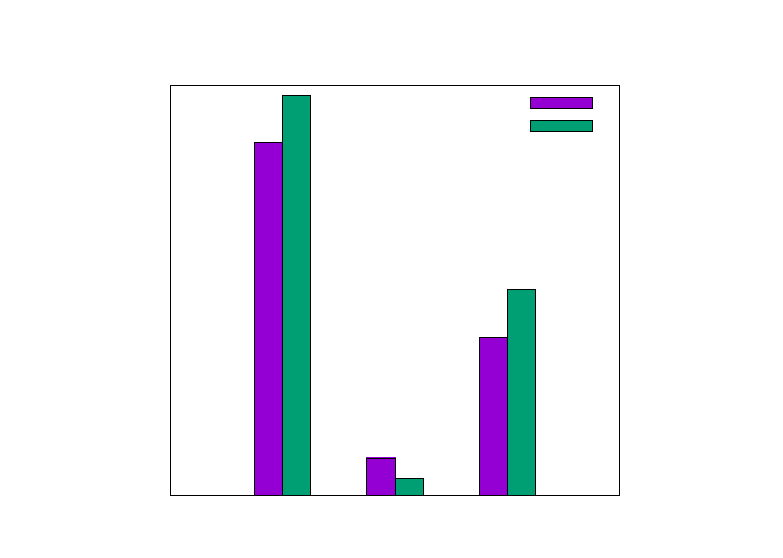
\includegraphics[width={360.00bp},height={252.00bp}]{efplot}}%
    \gplfronttext
  \end{picture}%
\endgroup

			}
			\caption{Space consumption and query time (for \numprint{1000000} predecessor queries) for my implementation of Elias-Fano. The three files are the three provided benchmark files.}
			\label{fig:ef}
		\end{center}
	\end{figure}

	\paragraph*{Range-Minimum Queries}
	Figure~\ref{fig:rmq} visualises the performance of the RMQ data structures, namely the two with~$\mathcal{O}\left(n \log n\right)$ and~$\mathcal{O}\left(n\right)$ additional memory consumption. The data structure with~$\mathcal{O}\left(n^2\right)$ memory consumption could not be executed due to too high memory consumption. It can be seen that the memory consumption between the two DSs is very different, namely, as expected, with significantly less memory for the DS with linear memory overhead. Interestingly, the query performance varies significantly between the DS with linear memory overhead because the ranges in the second file are relatively small. In my implementation, this only calls a local sequential search, which is the most cache-efficient and, for small ranges, the fastest way. Otherwise, the query performance of the~$\mathcal{O}\left(n \log n\right)$ DS does not depend on the range since the query performs lookups ``independent'' of the given range.
	\begin{figure}[htbp]
		\begin{center}
			\resizebox{.9\linewidth}{!}{
				% GNUPLOT: LaTeX picture with Postscript
\begingroup
  \makeatletter
  \providecommand\color[2][]{%
    \GenericError{(gnuplot) \space\space\space\@spaces}{%
      Package color not loaded in conjunction with
      terminal option `colourtext'%
    }{See the gnuplot documentation for explanation.%
    }{Either use 'blacktext' in gnuplot or load the package
      color.sty in LaTeX.}%
    \renewcommand\color[2][]{}%
  }%
  \providecommand\includegraphics[2][]{%
    \GenericError{(gnuplot) \space\space\space\@spaces}{%
      Package graphicx or graphics not loaded%
    }{See the gnuplot documentation for explanation.%
    }{The gnuplot epslatex terminal needs graphicx.sty or graphics.sty.}%
    \renewcommand\includegraphics[2][]{}%
  }%
  \providecommand\rotatebox[2]{#2}%
  \@ifundefined{ifGPcolor}{%
    \newif\ifGPcolor
    \GPcolorfalse
  }{}%
  \@ifundefined{ifGPblacktext}{%
    \newif\ifGPblacktext
    \GPblacktexttrue
  }{}%
  % define a \g@addto@macro without @ in the name:
  \let\gplgaddtomacro\g@addto@macro
  % define empty templates for all commands taking text:
  \gdef\gplbacktext{}%
  \gdef\gplfronttext{}%
  \makeatother
  \ifGPblacktext
    % no textcolor at all
    \def\colorrgb#1{}%
    \def\colorgray#1{}%
  \else
    % gray or color?
    \ifGPcolor
      \def\colorrgb#1{\color[rgb]{#1}}%
      \def\colorgray#1{\color[gray]{#1}}%
      \expandafter\def\csname LTw\endcsname{\color{white}}%
      \expandafter\def\csname LTb\endcsname{\color{black}}%
      \expandafter\def\csname LTa\endcsname{\color{black}}%
      \expandafter\def\csname LT0\endcsname{\color[rgb]{1,0,0}}%
      \expandafter\def\csname LT1\endcsname{\color[rgb]{0,1,0}}%
      \expandafter\def\csname LT2\endcsname{\color[rgb]{0,0,1}}%
      \expandafter\def\csname LT3\endcsname{\color[rgb]{1,0,1}}%
      \expandafter\def\csname LT4\endcsname{\color[rgb]{0,1,1}}%
      \expandafter\def\csname LT5\endcsname{\color[rgb]{1,1,0}}%
      \expandafter\def\csname LT6\endcsname{\color[rgb]{0,0,0}}%
      \expandafter\def\csname LT7\endcsname{\color[rgb]{1,0.3,0}}%
      \expandafter\def\csname LT8\endcsname{\color[rgb]{0.5,0.5,0.5}}%
    \else
      % gray
      \def\colorrgb#1{\color{black}}%
      \def\colorgray#1{\color[gray]{#1}}%
      \expandafter\def\csname LTw\endcsname{\color{white}}%
      \expandafter\def\csname LTb\endcsname{\color{black}}%
      \expandafter\def\csname LTa\endcsname{\color{black}}%
      \expandafter\def\csname LT0\endcsname{\color{black}}%
      \expandafter\def\csname LT1\endcsname{\color{black}}%
      \expandafter\def\csname LT2\endcsname{\color{black}}%
      \expandafter\def\csname LT3\endcsname{\color{black}}%
      \expandafter\def\csname LT4\endcsname{\color{black}}%
      \expandafter\def\csname LT5\endcsname{\color{black}}%
      \expandafter\def\csname LT6\endcsname{\color{black}}%
      \expandafter\def\csname LT7\endcsname{\color{black}}%
      \expandafter\def\csname LT8\endcsname{\color{black}}%
    \fi
  \fi
    \setlength{\unitlength}{0.0500bp}%
    \ifx\gptboxheight\undefined%
      \newlength{\gptboxheight}%
      \newlength{\gptboxwidth}%
      \newsavebox{\gptboxtext}%
    \fi%
    \setlength{\fboxrule}{0.5pt}%
    \setlength{\fboxsep}{1pt}%
    \definecolor{tbcol}{rgb}{1,1,1}%
\begin{picture}(7200.00,5040.00)%
    \gplgaddtomacro\gplbacktext{%
      \csname LTb\endcsname%%
      \put(1342,440){\makebox(0,0)[r]{\strut{}$8\times10^{7}$}}%
      \put(1342,878){\makebox(0,0)[r]{\strut{}$1\times10^{8}$}}%
      \put(1342,1315){\makebox(0,0)[r]{\strut{}$1.2\times10^{8}$}}%
      \put(1342,1753){\makebox(0,0)[r]{\strut{}$1.4\times10^{8}$}}%
      \put(1342,2191){\makebox(0,0)[r]{\strut{}$1.6\times10^{8}$}}%
      \put(1342,2628){\makebox(0,0)[r]{\strut{}$1.8\times10^{8}$}}%
      \put(1342,3066){\makebox(0,0)[r]{\strut{}$2\times10^{8}$}}%
      \put(1342,3504){\makebox(0,0)[r]{\strut{}$2.2\times10^{8}$}}%
      \put(1342,3941){\makebox(0,0)[r]{\strut{}$2.4\times10^{8}$}}%
      \put(1342,4379){\makebox(0,0)[r]{\strut{}$2.6\times10^{8}$}}%
      \put(2869,220){\makebox(0,0){\strut{}ex1.txt}}%
      \put(4264,220){\makebox(0,0){\strut{}ex2.txt}}%
      \put(5791,440){\makebox(0,0)[l]{\strut{}$0$}}%
      \put(5791,1228){\makebox(0,0)[l]{\strut{}$5000$}}%
      \put(5791,2016){\makebox(0,0)[l]{\strut{}$10000$}}%
      \put(5791,2803){\makebox(0,0)[l]{\strut{}$15000$}}%
      \put(5791,3591){\makebox(0,0)[l]{\strut{}$20000$}}%
      \put(5791,4379){\makebox(0,0)[l]{\strut{}$25000$}}%
    }%
    \gplgaddtomacro\gplfronttext{%
      \csname LTb\endcsname%%
      \put(209,2409){\rotatebox{-270}{\makebox(0,0){\strut{}Space [bits]}}}%
      \put(6693,2409){\rotatebox{-270}{\makebox(0,0){\strut{}Time [ms]}}}%
      \csname LTb\endcsname%%
      \put(4672,4206){\makebox(0,0)[r]{\strut{}N Space [bits]}}%
      \csname LTb\endcsname%%
      \put(4672,3986){\makebox(0,0)[r]{\strut{}N Time [ms]}}%
      \csname LTb\endcsname%%
      \put(4672,3766){\makebox(0,0)[r]{\strut{}N Log N Space [bits]}}%
      \csname LTb\endcsname%%
      \put(4672,3546){\makebox(0,0)[r]{\strut{}N Log N Time [ms]}}%
      \csname LTb\endcsname%%
      \put(3566,4709){\makebox(0,0){\strut{}Space and Time}}%
    }%
    \gplbacktext
    \put(0,0){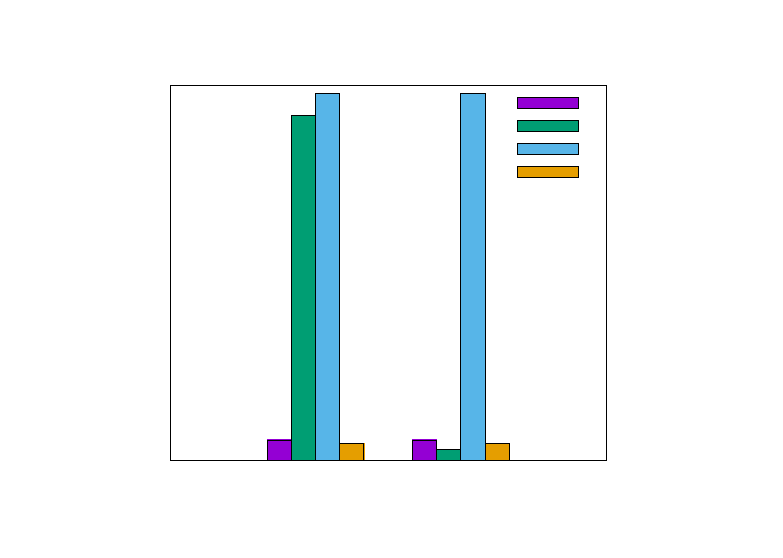
\includegraphics[width={360.00bp},height={252.00bp}]{rmqplot}}%
    \gplfronttext
  \end{picture}%
\endgroup

			}
			\caption{Shown is the memory consumption and performance of the range-minimum query data structures \textit{N Log N} and \textit{N} on the benchmark files. Note: the~$\mathcal{O}\left(n^2\right)$ data structure could not be executed on the benchmarks due to high memory consumption.}
			\label{fig:rmq}
		\end{center}
	\end{figure}
	
	\bibliography{bib}
	
	\appendix
	\section{A Note on Elias-Fano}
	\label{app:sec::ef}
	In the script, the first~$\left\lceil \log\left(n\right)\right\rceil$ bits were defined as MSB, but this definition caused problems with \eg the following numbers:
	
	\begin{equation*}
		0, 1, 10, 13, 32, 64, \numprint{1926720561250547757}, \numprint{4354482840745948438}, \numprint{18446013172173323708}
	\end{equation*}
	Now, looking at the various MSBs of length~$\left\lceil \log\left(n\right)\right\rceil = 4$, we see:
	
	\begin{equation}
		\left(0000\right)_2, \left(0001\right)_2, \left(0011\right)_2, \left(1111\right)_2
	\end{equation}
	
	If \textit{upperBits} has a length of~$2\cdot9+1 = 19$, then to decode the last number, you would need to acces the index~$\left(1111\right)_2 + 8 = 23$, which is out of bounds for \textit{upperBits}. Therefore, I set the length of the \textit{upperBits} to~$3 \cdot n$, as discussed in the lecture.
\end{document}
